\documentclass[11pt]{article}
\usepackage[utf8]{inputenc}  
\usepackage[T1]{fontenc}     
\usepackage{lmodern}         
\usepackage{microtype}       
\usepackage{geometry}        
\usepackage{amsmath, amssymb} 
\usepackage{graphicx}        
\usepackage{hyperref}        
\usepackage{enumitem}        
\usepackage{xcolor}          
\usepackage{tcolorbox}       
\usepackage{accents}
\usepackage{tikz}
\usepackage{stmaryrd}
\usepackage{caption}
\usepackage{multicol}
\usepackage{blindtext}
\usepackage{breqn}
\usepackage{titlesec}
\usepackage[parfill]{parskip} 
\usetikzlibrary{patterns}
\hypersetup{
    colorlinks = false,
    linkbordercolor = {white},
}

%From M275 "Topology" at SJSU
\newcommand{\id}{\mathrm{id}}
\newcommand{\taking}[1]{\xrightarrow{#1}}
\newcommand{\inv}{^{-1}}
\usepackage{accents}
\usepackage{bbold}

%From M170 "Introduction to Graph Theory" at SJSU
\DeclareMathOperator{\diam}{diam}
\DeclareMathOperator{\ord}{ord}
\newcommand{\defeq}{\overset{\mathrm{def}}{=}}

%From the USAMO .tex files
\newcommand{\ts}{\textsuperscript}
\newcommand{\dg}{^\circ}
\newcommand{\ii}{\item}

% % From Math 55 and Math 145 at Harvard
% \newenvironment{subproof}[1][Proof]{%
% \begin{proof}[#1] \renewcommand{\qedsymbol}{$\blacksquare$}}%
% {\end{proof}}

\newcommand{\liff}{\leftrightarrow}
\newcommand{\lthen}{\rightarrow}
\newcommand{\opname}{\operatorname}
\newcommand{\surjto}{\twoheadrightarrow}
\newcommand{\injto}{\hookrightarrow}
\newcommand{\On}{\mathrm{On}} % ordinals
\DeclareMathOperator{\img}{im} % Image
\DeclareMathOperator{\Img}{Im} % Image
\DeclareMathOperator{\coker}{coker} % Cokernel
\DeclareMathOperator{\Coker}{Coker} % Cokernel
\DeclareMathOperator{\Ker}{Ker} % Kernel
\DeclareMathOperator{\rank}{rank}
\DeclareMathOperator{\Spec}{Spec} % spectrum
\DeclareMathOperator{\Tr}{Tr} % trace
\DeclareMathOperator{\pr}{pr} % projection
\DeclareMathOperator{\ext}{ext} % extension
\DeclareMathOperator{\pred}{pred} % predecessor
\DeclareMathOperator{\dom}{dom} % domain
\DeclareMathOperator{\ran}{ran} % range
\DeclareMathOperator{\Hom}{Hom} % homomorphism
\DeclareMathOperator{\Mor}{Mor} % morphisms
\DeclareMathOperator{\End}{End} % endomorphism

\newcommand{\eps}{\epsilon}
\newcommand{\veps}{\varepsilon}
\newcommand{\ol}{\overline}
\newcommand{\ul}{\underline}
\newcommand{\wt}{\widetilde}
\newcommand{\wh}{\widehat}
\newcommand{\vocab}[1]{\textbf{\color{blue} #1}}
\providecommand{\half}{\frac{1}{2}}
\newcommand{\dang}{\measuredangle} %% Directed angle
\newcommand{\ray}[1]{\overrightarrow{#1}}
\newcommand{\seg}[1]{\overline{#1}}
\newcommand{\arc}[1]{\wideparen{#1}}
\DeclareMathOperator{\cis}{cis}
\DeclareMathOperator*{\lcm}{lcm}
\DeclareMathOperator*{\argmin}{arg min}
\DeclareMathOperator*{\argmax}{arg max}
\newcommand{\cycsum}{\sum_{\mathrm{cyc}}}
\newcommand{\symsum}{\sum_{\mathrm{sym}}}
\newcommand{\cycprod}{\prod_{\mathrm{cyc}}}
\newcommand{\symprod}{\prod_{\mathrm{sym}}}
\newcommand{\Qed}{\begin{flushright}\qed\end{flushright}}
\newcommand{\parinn}{\setlength{\parindent}{1cm}}
\newcommand{\parinf}{\setlength{\parindent}{0cm}}
% \newcommand{\norm}{\|\cdot\|}
\newcommand{\inorm}{\norm_{\infty}}
\newcommand{\opensets}{\{V_{\alpha}\}_{\alpha\in I}}
\newcommand{\oset}{V_{\alpha}}
\newcommand{\opset}[1]{V_{\alpha_{#1}}}
\newcommand{\lub}{\text{lub}}
\newcommand{\del}[2]{\frac{\partial #1}{\partial #2}}
\newcommand{\Del}[3]{\frac{\partial^{#1} #2}{\partial^{#1} #3}}
\newcommand{\deld}[2]{\dfrac{\partial #1}{\partial #2}}
\newcommand{\Deld}[3]{\dfrac{\partial^{#1} #2}{\partial^{#1} #3}}
\newcommand{\lm}{\lambda}
\newcommand{\uin}{\mathbin{\rotatebox[origin=c]{90}{$\in$}}}
\newcommand{\usubset}{\mathbin{\rotatebox[origin=c]{90}{$\subset$}}}
\newcommand{\lt}{\left}
\newcommand{\rt}{\right}
\newcommand{\bs}[1]{\boldsymbol{#1}}
\newcommand{\exs}{\exists}
\newcommand{\dps}[1]{\displaystyle{#1}}

\newcommand{\sol}{\setlength{\parindent}{0cm}\textbf{\textit{Solution:}}\setlength{\parindent}{1cm} }
\newcommand{\solve}[1]{\setlength{\paraindent}{0cm}\textbf{\textit{Solution: }}\setlength{\parindent}{1cm}#1 \Qed}

\newcommand{\middleline}{
    \par\noindent\raisebox{.5\baselineskip}{\makebox[\linewidth]{\rule{0.5\textwidth}{0.4pt}}}\par
}

\newcommand{\calC}{\mathcal{C}}
\newcommand{\st}{\text{s.t.}}
\newcommand{\calD}{\mathcal{D}} 
\newcommand{\calB}{\mathcal{B}}
% Theorems 
% Define theorem-like environments
\newtheorem{lemma}{Lemma}[section]
\newtheorem{proposition}[lemma]{Proposition}
\newtheorem{definition}[lemma]{Definition}
\newtheorem{example}[lemma]{Example}
\newenvironment{proof}{\paragraph{Proof:}}{\hfill$\square$}
%%%%%%%%%%%%%%%%%%%%%%%%%%%%%%%%%%%%%%%%%%%%%%%%%%
% Begin macro definitions
%%%%%%%%%%%%%%%%%%%%%%%%%%%%%%%%%%%%%%%%%%%%%%%%%%

%%%%%%%%%%%%%%%%%%%%%%%%%%%%%%%%%%%%%%%%%%%%%%%%%%
% Matthew's new ones:
\newcommand{\model}{\text{Mod}}
\newcommand\subsetsim{\mathrel{\substack{\textstyle\sqsubset\\[-0.2ex]\textstyle\sim}}}

%%%%%%%%%%%%%%%%%%%%%%%%%%%%%%%%%%%%%%%%%%%%%%%%%%
% General expressions and commands:

\newcommand{\ie}{\mbox{i.e.}}
\newcommand{\eg}{\mbox{e.g.}}
\newcommand{\cf}{\mbox{cf.}}
\newcommand{\viz}{\mbox{viz.}}
\newcommand{\wrt}{\mbox{w.r.t.}}
\newcommand{\wolog}{\mbox{w.l.o.g.}}
\newcommand{\etal}{\mbox{et al}}
\newcommand{\vs}{\mbox{vs.}}
\newcommand{\aka}{\mbox{a.k.a.}}
\newcommand{\myskip}{\medskip} % space interlines

%%%%%%%%%%%%%%%%%%%%%%%%%%%%%%%%%%%%%%%%%%%%%%%%%%
% Mathematical general expressions:

%\newcommand{\qed}{\rule{2mm}{2mm}}
\newcommand{\tuple}[1]{\langle #1 \rangle}
\newcommand{\defined}{\ensuremath{\equiv_{\text{def}}}}
\newcommand{\abbrev}{\mathrel{\mathop:}=}
\newcommand{\eqclass}[1]{[#1]} % equivalence class of an element

%%%%%%%%%%%%%%%%%%%%%%%%%%%%%%%%%%%%%%%%%%%%%%%%%%
% Theorem-like environments:

%\newtheorem{definition}{Definition}
%\let\olddefinition\definition
%\renewcommand{\definition}{\olddefinition\normalfont}

%\newtheorem{lemma}{Lemma}%[section]
%\newtheorem{theorem}{Theorem}%[section] 
%\newtheorem{proposition}{Proposition}%[section]
%\newtheorem{corollary}{Corollary}%[section]

%\newtheorem{example}{Example}%[section]%}
%\let\oldexample\example
%\renewcommand{\example}{\oldexample\normalfont}

%\newtheorem{remark}{Remark}%[section]
\newtheorem{observation}{Observation}%[section]
%\newenvironment{proof}{\noindent\textbf{Proof:}\null\hfill\null\newline}{\hfill\qed}

%%%%%%%%%%%%%%%%%%%%%%%%%%%%%%%%%%%%%%%%%%%%%%%%%%
% Computational complexity:

\newcommand{\ptime}{\textsc{P}}
\newcommand{\np}{\textsc{NP}}
\newcommand{\exptime}{\textsc{exptime}}
\newcommand{\pspace}{\textsc{pspace}}
\newcommand{\npcomplete}{\textsc{np-complete}}

%%%%%%%%%%%%%%%%%%%%%%%%%%%%%%%%%%%%%%%%%%%%%%%%%%
% Sets and set operations:

% Set union: \cup, Set intersection: \cap, Set difference: \setminus
\newcommand{\powerset}[1]{\mathscr{P}(#1)} % powerset
\newcommand{\symdiff}{\dotdiv} % symmetric difference

%%%%%%%%%%%%%%%%%%%%%%%%%%%%%%%%%%%%%%%%%%%%%%%%%%
% Special sets:

% Language:
\newcommand{\Prp}{\ensuremath{\mathcal{P}}}
\newcommand{\Lang}{\ensuremath{\mathcal{L}}}

% Theories, signature:
\newcommand{\T}{\ensuremath{\mathcal{T}}} % a theory
\newcommand{\KB}{\ensuremath{\mathcal{K}}} % a knowledge base
\newcommand{\Sig}{\ensuremath{\mathcal{S}}} % a set of atoms, or a signature
% Theories, signature:
\newcommand{\A}{\ensuremath{\mathcal{A}}} % an ABox
\newcommand{\calO}{\ensuremath{\mathcal{K}_\mathcal{I}}}% a set of individuals
%%%%%%%%%%%%%%%%%%%%%%%%%%%%%%%%%%%%%%%%%%%%%%%%%%
% Logical connectives and meta-logical basic definitions:

% Logical negation: \lnot, Logical conjunction: \land, Logical disjunction: \lor
\newcommand{\limp}{\rightarrow} % logical implication
\newcommand{\lexor}{\oplus} % exclusive or

% Entailment  in a class of models:
\newcommand{\Centails}[1]{\models_{\raisebox{-0.25ex}{$\!\!\!_{#1}$}}\!\!}
\newcommand{\nCentails}{\not\Centails}

% Provable in a given logical system:
\newcommand{\provable}[1]{\vdash_{\raisebox{-0.2ex}{$\!\!\!_{#1}$}}\!\!}
\newcommand{\nprovable}[1]{\not\provable{#1}}

%%%%%%%%%%%%%%%%%%%%%%%%%%%%%%%%%%%%%%%%%%%%%%%%%%
% Classical Propositional Logic:

\newcommand{\verum}{\ensuremath{\text{\it true}}}
\newcommand{\falsum}{\ensuremath{\text{\it false}}}
\newcommand{\fml}{\ensuremath{\varphi}} % a classical formula
\newcommand{\clause}{\ensuremath{\chi}} % a clause
\newcommand{\term}{\ensuremath{\pi}} % a term
\newcommand{\Val}{\ensuremath{\mathcal{V}}} % set of propositional valuations

% Satisfaction relation:
\newcommand{\sat}{\Vdash}
\newcommand{\nsat}{\not\sat}

% Classical propositional entailment:
\newcommand{\entails}{\models}
\newcommand{\nentails}{\not\entails}
\newcommand{\entailed}{\raisebox{1.1ex}{\rotatebox{180}{$\entails$}}}

% Classical provability:
\newcommand{\proves}{\vdash}
\newcommand{\nproves}{\not\proves}

% Propositional consequence relation and provability:
\newcommand{\CPL}{{\sf CPL}}
\newcommand{\CPLentails}{\Centails{\CPL}}
\newcommand{\nCPLentails}{\not\CPLentails}
\newcommand{\CPLtheorem}{\provable{\CPL}}
\newcommand{\nCPLtheorem}{\not\CPLtheorem}

%%%%%%%%%%%%%%%%%%%%%%%%%%%%%%%%%%%%%%%%%%%%%%%%%%
% Modal logic:

% Modal operators:
\newcommand{\nec}{\Box}
\newcommand{\poss}{\Diamond}
\newcommand{\Nec}[1]{[ #1 ]}
\newcommand{\Poss}[1]{\langle #1 \rangle}
\newcommand{\obl}{\scalebox{0.75}{\raisebox{0.5ex}{\ensuremath{\bigcirc}}}} % obligation

% Kripke models:
\newcommand{\W}{\ensuremath{\text{\it W}}} % possible worlds
\newcommand{\R}{\ensuremath{\text{\it R}}} % accessibility relation
\newcommand{\V}{\ensuremath{\text{\it V}}} % valuation function
\newcommand{\M}{\mathscr{M}}
\newcommand{\MSet}{\ensuremath{\mathcal{M}}} % set of models
\newcommand{\USet}{\mathcal{U}} % set of pointed models

% Valid in a given model:
\newcommand{\Mvalid}[1]{\models^{\raisebox{-0.3ex}{$\!\!\!^{#1}$}}\!\!}
\newcommand{\nMvalid}[1]{\not\Mvalid{#1}}

% Modal logic K:
\newcommand{\Kentails}{\Centails{\K}}
\newcommand{\nKentails}{\not\Kentails}
\newcommand{\Ktheorem}{\provable{\K}}
\newcommand{\nKtheorem}{\not\Ktheorem}
\newcommand{\schemaK}{\ensuremath{\text{{\it K}}}}
\newcommand{\ruleRN}{\ensuremath{\text{{\it RN}}}}

%%%%%%%%%%%%%%%%%%%%%%%%%%%%%%%%%%%%%%%%%%%%%%%%%%
% Description Logics:

\newcommand{\N}{\ensuremath{{\sf N}}} % set of concept names
\newcommand{\CN}{\ensuremath{{\sf N}_{\mathscr{C}}}} % set of concept names
\newcommand{\RN}{\ensuremath{{\sf N}_{\mathscr{R}}}} % set of role names
\newcommand{\IN}{\ensuremath{{\sf N}_{\mathscr{I}}}} % set of individual names
\newcommand{\Names}{\ensuremath{{\sf N}}}  % union of both (the whole signature)
\newcommand{\dlAnd}{\sqcap}
\newcommand{\dlOr}{\sqcup}
\newcommand{\subs}{\sqsubseteq}
\newcommand{\nsubs}{\not\subs}
\newcommand{\I}{\ensuremath{\mathcal{I}}}
\newcommand{\J}{\ensuremath{\mathcal{J}}}
\newcommand{\Iof}[1]{{#1}^{\I}}
\newcommand{\Db}{\mathcal{D}}
\newcommand{\Dom}{\Delta}
\newcommand{\Ifunc}{\Iof{\cdot}}
\newcommand{\ALC}{\ensuremath{\mathcal{ALC}}}
\newcommand{\SHIF}{\ensuremath{\mathcal{SHIF}}}
\newcommand{\SHOIN}{\ensuremath{\mathcal{SHOIN}}}
\newcommand{\EL}{\ensuremath{\mathcal{EL}}}
\newcommand{\ABox}{\ensuremath{\mathcal{A}}}
\newcommand{\Ont}{\ensuremath{\mathcal{O}}}

\newcommand{\CSet}{\ensuremath{\mathcal{C}}}


% Concept and role names:
\newcommand{\NPP}{{\sf NuclearPP}}
\newcommand{\AtomicPile}{{\sf AtomicPile}}
\newcommand{\rNPP}{{\sf RiskyNPP}}
\newcommand{\BrNPP}{{\sf BrazilianNPP}}
\newcommand{\Brazil}{{\sf Brazil}}
\newcommand{\Safe}{{\sf Safe}}
\newcommand{\SeismicArea}{{\sf SeismicArea}}
\newcommand{\isLocated}{{\sf isLocated}}
\newcommand{\hasComponent}{{\sf hasComponent}}
\newcommand{\meltDown}{{\sf meltDown}}
\newcommand{\marriedTo}{{\sf marriedTo}}
\newcommand{\partOf}{{\sf partOf}}
\newcommand{\parentOf}{{\sf parentOf}}
\newcommand{\progenitorOf}{{\sf progenitorOf}}
\newcommand{\worksFor}{{\sf worksFor}}
\newcommand{\bird}{{\sf b}}
\newcommand{\penguin}{{\sf p}}
\newcommand{\flies}{{\sf f}}
\newcommand{\wings}{{\sf w}}
\newcommand{\nbird}{\overline{\sf b}}
\newcommand{\npenguin}{\overline{\sf p}}
\newcommand{\nflies}{\overline{\sf f}}
\newcommand{\nwings}{\overline{\sf w}}
\newcommand{\p}{\sf p}
\newcommand{\q}{\sf q}
\newcommand{\notp}{\overline{\sf p}}
\newcommand{\notq}{\overline{\sf q}}


%%%%%%%%%%%%%%%%%%%%%%%%%%%%%%%%%%%%%%%%%%%%%%%%%%
% Special functions and relations:

% Range of a function or relation:
\newcommand{\range}[1]{{\ensuremath{\text{\it range}(#1)}}}
% Domain of a function or relation:
\newcommand{\domain}[1]{{\ensuremath{\text{\it domain}(#1)}}}
% Atoms of a formula:
\newcommand{\atm}[1]{{\ensuremath{\text{\it atm}(#1)}}}
% Literals of a formula:
\newcommand{\lit}[1]{{\ensuremath{\text{\it lit}(#1)}}}
% Symbols in a formula:
\newcommand{\sig}[1]{{\ensuremath{\text{\it sig}(#1)}}}
% Cardinality of a set:
\newcommand{\card}[1]{{\ensuremath{\text{\it card}(#1)}}}
% Models of a formula:
\newcommand{\Mod}[1]{{\ensuremath{\text{\it Mod}(#1)}}}
% Logical consequences of a theory:
\newcommand{\Cn}[1]{{\ensuremath{\text{\it Cn}(#1)}}}
\newcommand{\Cns}[2]{{\ensuremath{\text{\it Cn}_{#1}(#2)}}}

%%%%%%%%%%%%%%%%%%%%%%%%%%%%%%%%%%%%%%%%%%%%%%%%%%
% Defeasible Stuff:

\newcommand{\dentails}{\mid\hskip-0.40ex\approx}
\newcommand{\ndentails}{\not\mid\hskip-0.40ex\approx}
\renewcommand{\bar}[1]{\overline{#1}}
\newcommand{\twiddle}{\mathrel|\joinrel\sim}
\newcommand{\ntwiddle}{\not\twiddle}
%\newcommand{\usually}{\raisebox{-0.5ex}{$\:\stackrel{\sqsubset}{{\scriptstyle\sim}}\:$} }
\newcommand{\usually}{\:\raisebox{0.45ex}{\ensuremath{\sqsubset}}\hskip-1.7ex\raisebox{-0.6ex}{\scalebox{0.9}{\ensuremath{\sim}}}\:}
\newcommand{\nusually}{\not\hspace{-1.1mm}\usually}
%\newcommand{\usuallyeq}{\raisebox{1.5ex}{\rotatebox{180}{$\cong$}}}
%\newcommand{\nusuallyeq}{\not\hspace{-1.1mm}\usuallyeq}
% Preferential models:
\newcommand{\St}{\ensuremath{\text{\it S}}} % set of states
\newcommand{\lab}{\ensuremath{\ell}} % labeling function
\newcommand{\pref}{\prec} % preference relation
\newcommand{\npref}{\not\pref}
\newcommand{\PM}{\mathscr{P}} % preferential model
\newcommand{\RM}{\mathscr{R}} % ranked model
\newcommand{\CM}{\mathscr{C}} % coherent ranked model
\newcommand{\RSet}{\ensuremath{\mathcal{R}}} % set of ranked models
\newcommand{\Rentails}{\Centails{\RSet}} % entailment in the class of ranked models
\newcommand{\nRentails}{\not\Rentails}
\newcommand{\Sat}{\mathrel|\joinrel\equiv} % satisfaction by a state
\newcommand{\nSat}{\not\Sat}
\newcommand{\states}[1]{\llbracket#1\rrbracket} % requires package stmaryrd
\newcommand{\rk}{\ensuremath{\text{\it rk}}} % ranking function
\newcommand{\nme}{\ensuremath{\mathscr{R}}} % relation of being not more exceptional than
%\newcommand{\C}{\ensuremath{\mathscr{C}}} % set of consistent concepts
\newcommand{\RC}{\ensuremath{\mathcal{R}^{\twiddle}}} % rational closure
\newcommand{\rel}{\ensuremath{\text{\it R}}} % binary relation on the domain
\newcommand{\sel}{{\ensuremath{\text{\sf sel}}}} % selection function

\newcommand{\OI}{\ensuremath{\mathcal{O}}} % ordered interpretation
\newcommand{\PI}{\ensuremath{\mathcal{P}}} % preferential interpretation
\newcommand{\RI}{\ensuremath{\mathcal{R}}} % ranked interpretation
\newcommand{\dsrel}{\leadsto}
\newcommand{\ndsrel}{\not\dsrel}
\newcommand{\D}{\ensuremath{\mathcal{D}}} % a defeasible TBox
\newcommand{\K}{\widetilde{\mathbb{K}}}
\newcommand{\Rs}{\mathscr{R}} % set of ranked models with same classical \I
\newcommand{\X}{\mathcal{X}} % variable for defeasible entailment subscript
\newcommand{\generalent}{\entails_{\X}} %subscripted entailment, based on variable \X

% Definitions for flag and flame (defeasible modal operators):
\newcommand*{\myleftmid}{%
      \mathrel{\vcenter{\offinterlineskip
      \vskip-0.25ex\hbox{$\shortmid$}}}}
\newcommand*{\myrightmid}{%
      \mathrel{\vcenter{\offinterlineskip
      \vskip-0.7ex\hbox{$\shortmid$}}}}
\newcommand*{\twosim}{%
      \mathrel{\vcenter{\offinterlineskip
      \vskip0.05ex\hbox{$\sim$}\vskip0.25ex\hbox{$\sim$}}}}
\newcommand{\bartwosim}{\mathrel{\myleftmid}\hskip-0.03ex\joinrel\twosim}
% Defeasible necessity:
\newcommand{\dnec}{\mathrel{\bartwosim}\hskip-.05ex\joinrel\myrightmid}
% Defeasible possibility:
\newcommand{\dposs}{\scalebox{0.8}{\raisebox{-0.2ex}{\rotatebox{57}{\ensuremath{\dnec}}}}\hskip-0.3ex}
% Defeasible obligation:
\newcommand{\smallsim}{\scalebox{0.86}{\raisebox{0.4ex}{\ensuremath{\sim}}}}
\newcommand{\dobl}{\mathrel{\obl}\hskip-1.9ex\joinrel\smallsim\hskip0.2ex}
% Language with defeasible modalities:
\newcommand{\Langd}{\widetilde{\Lang}}
% Defeasible quantifiers:
\newcommand{\smallsimforall}{\scalebox{0.68}{\raisebox{0.76ex}{\ensuremath{\sim}}}}
\newcommand{\dforall}{\forall\hskip-1.06ex\raisebox{0.7ex}{\scalebox{0.7}{\ensuremath{\textcolor{white}{\bullet}}}}\hskip-1.88ex\joinrel\smallsimforall}
\newcommand{\smallsimexists}{\scalebox{0.65}{\raisebox{0.62ex}{\ensuremath{\sim}}}}
\newcommand{\dexists}{\exists\hskip-1.5ex\scalebox{1.2}{\ensuremath{\textcolor{white}{\bullet}}}\hskip-2.05ex\joinrel\smallsimexists}

\newcommand{\ratent}{\vdash_{r}}

\newcommand{\minent}{\entails_R^{\cup}}
\newcommand{\ratentabox}{\vdash_{r}}
\newcommand{\tw}[1]{\widetilde{#1}}
\newcommand{\E}{\ensuremath{\mathcal{E}}} % exceptionality function
\newcommand{\e}{\ensuremath{\varepsilon}} % exceptionality function
%\newtheorem{procedure}{
%[section]

%%%%%%%%%%%%%%%%%%%%%%%%%%%%%%%%%%%%%%%%%%%%%%%%%%
% Miscellaneous:

% Global options:
%\renewcommand{\labelitemi}{{\small\textbullet}}
%\renewcommand\arraystretch{1.5}
%\renewcommand{\familydefault}{\sfdefault} % sets font to sans serif globally 

% Useful commands:
\newcommand{\nil}{\textcolor{white}{a}} 
\newcommand{\hide}[1]{}
\newcommand{\red}[1]{\textcolor{red}{#1}}
%\newcommand{\todo}[1]{\textcolor{red}{\underline{{\sf #1}} $\blacktriangleright$}}
%\newcommand{\note}[1]{\textcolor{green}{\underline{{\sf #1}} $\blacktriangleright$}}
\newcommand{\who}[1]{\textcolor{orange}{\underline{{\sf #1}} $\blacktriangleright$}}
% Rounded white box with orange frame:
\newlength{\RoundedBoxWidth}
\newsavebox{\WhiteRoundedBox}
\newenvironment{WhiteBox}[1][\dimexpr\textwidth-4.5ex]%
   {\setlength{\RoundedBoxWidth}{\dimexpr#1}
    \begin{lrbox}{\WhiteRoundedBox}
       \begin{minipage}{\RoundedBoxWidth}}%
   {   \end{minipage}
    \end{lrbox}
    \begin{center}
    
\begin{tikzpicture}%
       \draw node[draw=Orange,fill=white,rounded corners,line width=1.5pt,%
             inner sep=0.7ex,text width=\RoundedBoxWidth]%
             {\usebox{\WhiteRoundedBox}};
    \end{tikzpicture}
    \end{center}}

\newcommand{\cass}[2]{\mbox{$#1:#2$}}
\newcommand{\rass}[3]{\mbox{$(#1,#2):#3$}}
\newcommand{\underlinesymbol}[1]{\underline{#1}}
\newcommand{\DCl}[1]{(\underlinesymbol{#1}^\circ)^\circ}
%%%%%%%%%%%%%%%%%%%%%%%%%%%%%%%%%%%%%%%%%%%%%%%%%%
% End macro definitions
%%%%%%%%%%%%%%%%%%%%%%%%%%%%%%%%%%%%%%%%%%%%%%%%%%

\geometry{
  a4paper,
  left=0.75in,
  right=0.75in,
  top=0.75in,
  bottom=0.75in,
}
\title{Defeasibility in Formal Concept Analysis}
\author{Lucas Carr}
\date{06.06.24 - }

\begin{document}
\maketitle
\tableofcontents
\clearpage

\section{Establishing Requirements}
\subsection{A defeasible formal context}
A regular formal context $\mathbb{K}$ is a tripple $(G,M,I)$ of objects $G$, attributes $M$, and an incidence relation $I \subseteq G \times M$. We define a defeasible formal context $\K$ as a quadruple $(G,M,I,\leq)$ with $G,M,I$ as before, and $\leq$ being a partial order on the objects $G$.

The ordering on $G$ can be loosely thought of as expressing a preference on objects such that if $o_1 \leq o_2$ and $o_1 \not = o_2$, then $o_1$ is preferred to $o_2$, where $o_1, o_2 \in G$.

\subsection{Minimisation}
In formal context analysis, two operators are defined

\begin{align*}
  A^{\uparrow} := \{m \in M | \forall g \in A, (g,m) \in I\}   &  & A \subseteq G \\
  \\
  B^{\downarrow} := \{g \in G | \forall m \in B, (g,m) \in I\} &  & B \subseteq M
\end{align*}

Much of the time it is not necessary to distinguish between $\cdot^{\uparrow}$ and $\cdot^{\downarrow}$, and so $A'$ and $B'$ are used instead.

We introduce a variation on these two operators, which has the same set building behavior, but discards any objects which are not minimal with respect to the partial order given by $\K$. The result is

\begin{align*}
  Min(O)                     & := \{g \in O | \nexists h \in O, h < g \} & O \subseteq G \\
  \\
  \underline{A^{\uparrow}}   & := (Min(A))^{\uparrow}                    & A \subseteq G \\
  \\
  \underline{B^{\downarrow}} & := Min(B^{\downarrow})                    & B \subseteq M
\end{align*}

When applied to a set of objects $A \subseteq G$, the minimisation operator removes all non-minimal elements from $A$, and then takes $A^{\uparrow}$. This gives us the set of attributes common to all minimal objects from $A$. Conversely, when applied to a set of atttributes $B \subseteq M$, the minimisation operator takes $B^{\downarrow}$, and removes all non-minimal objects, leaving the minimal objects which have all the attributes from $B$ in their object intents.

Given a set of attributes $B \subseteq M$, we can determine $\underline{(\underline{B^{\downarrow}})^{\uparrow}}$ (although, this double minimisation is not strictly necessary, when applying the operator twice on an initial set of attributes $B\subseteq M$, we will omit the double minimisation, giving us $\dminO{B}$). This constructs the set of attribute which are common to all minimal objects which have $B$ in their object intents. We make this clear with an example


\subsubsection{Example}
The context $\K = (G,M,I,\leq)$ with the order over $G$ being $\{o_1 < o_3, o_2 < o_3, o_3 < o_4, o_5 < o_4\}$
\begin{figure}[h]
  \begin{center}
    \begin{tabular}{r|cccccc}
            & feathered & laysEggs & aquatic  & canFly   & hasScales \\ \hline
      $o_1$ &           & $\times$ & $\times$ &          & $\times$  \\
      $o_2$ & $\times$  & $\times$ & $\times$ & $\times$ & $$        \\
      $o_3$ &           & $\times$ & $\times$ &          & $\times$  \\
      $o_4$ & $\times$  & $\times$ & $$       & $\times$ & $$        \\
      $o_5$ & $\times$  & $\times$ & $$       & $$       & $$
    \end{tabular}
  \end{center}
  \caption{Defeasible Formal Context}
  \label{fig:defeasible-formal-context}
\end{figure}

Given the set of attributes $Y :=$\{\texttt{laysEggs}, \texttt{canFly}\}, our first application of the minimisation operator gives us $\minO{Y} = Min(\{o_2, o_4\}) = \{o_2\}$. Applying the operator again, to the first result, we get $\dminO{Y} = \minO{\{o_2\}} = \{\text{\texttt{feathered}, \texttt{laysEggs}, \texttt{aquatic}, \texttt{canFly}}\}$. Plainly, this tells us that the most preferred objects which can fly and lay eggs, also are feathered and aquatic.

\subsection{Properties of the minimisation-operator}
\label{subsection:properties-min-operator}
The $\cdot''$ operator in FCA is a closure-operator, so it is monotonic, extensive, and idempotent. In the following, we show that the minimisation-operator is nonmonotonic, extensive, and idempotent over sets of $M$ in a defeasible context $\K = (G,M,I,\leq)$.

\begin{proposition}
  \label{proposition-min_operator}
  The minimisation operator is nonmonotonic, extensive, and idempotent over sets of $M$.
\end{proposition}

\begin{proof}
  Nonmonotonicity, Extensivity, Idempotency of the minimisation operator.

  \textbf{Nonmonotonicity:}

  \begin{quotation}
    \noindent If $\dminO{\cdot}$ were monotonic, we would have $A \subseteq B \Rightarrow \dminO{A} \subseteq \dminO{B}$, with $A,B \subseteq M$. \\

    \noindent Let $\K$ be a defeasible context with two objects, $o_1$ and $o_2$, attributes $\{m_1, m_2, m_3, m_4\}$, and an ordering $o_1 < o_2$. The intents of each objects are $\{m_1, m_2, m_4\}$ and $\{m_1, m_2, m_3\}$, respectively. If we take the sets $A = \{m_1,m_2\}$ and $B = \{m_1, m_2, m_3\}$ we have that $A\subseteq B$. However, $\dminO{A} = \{m_1, m_2, m_4\}$ and $\dminO{B} = \{m_1, m_2, m_3\}$, and so $\dminO{A} \not \subseteq \dminO{B}$. Consequently, the minimisation operator is nonmonotonic.
  \end{quotation}

  \textbf{Extensivity:}
  \begin{quotation}
    \noindent For $A \subseteq M$, extensivity requires that $A \subseteq \dminO{A}$.\\

    \noindent We know that $A \subseteq A''$, since $\cdot''$ is extensive. So, for all $a \in A'$, we have that $A$ is in $a$ object intent $A \subseteq a'$. Since the minimisation operator simply reduces the size of $A'$, then $\minO{A} \subseteq A'$. So the earlier condition holds, that for all $a \in \minO{A}$ the object intent is a superset of $A$, or $A \subseteq a'$. From this, it is easy to see that $A \subseteq \bigcap \{a' | a \in \minO{A}\}$, and equivalently $A \subseteq \dminO{A}$.

  \end{quotation}

  \textbf{Idempotency:}
  \begin{quotation}
    \noindent The proof for idempotency follows from extensivity. Given some $A \subseteq M$, $\dminO{A}$ represents attributes of the minimal objects satisfying $A$. If $\dminO{A} \not =\dminO{(\dminO{A})}$, then we would have that there were some new minimal objects in $\minO{(\dminO{A})}$, these objects would all have $A$ in their intents by extensivity. But this is a contradiction, since $\dminO{A}$ is defined to be the minimal objects with $A$ in their intent, there can be no objects minimal $\minO{A}$ which also have $A$ in their intents.
  \end{quotation}
\end{proof}

\clearpage
\section{Defeasible Implications}
\subsection{Normal implications}
Conventionally, we define an implication $A\rightarrow B$ between two sets of attributes $A,B \subseteq M$. An implication is respected \footnote{being \textit{respected} is analagous to being entailed} in a formal context iff

\begin{itemize}
  \item $B \subseteq A''$
  \item $A' \subseteq B'$
\end{itemize}

An example from \autoref{fig:defeasible-formal-context} would be that $\texttt{canFly} \rightarrow \texttt{feathered}$. The objects which satisfy the attribute \texttt{canFly}, namely $\{o_2, o_4\}$, are a subset of those which satisfy \texttt{feathered}, $\{o_2, o_4, o_5\}$. We do not have that $\texttt{feathered} \rightarrow \texttt{canFly}$ - this is obvious, and can be shown by $\texttt{canFly} \not \subseteq \texttt{feathered}''$

\subsection{Borrowing the $\twiddle$}
In $\K = (G,M,I, <)$, we define a defeasible implication $A \twiddle B$, where $A,B \subseteq M$ as being respected in the $\K$ iff
\begin{itemize}
  \item $B \subseteq \dminO{A}$
  \item $\minO{A} \subseteq B'$
\end{itemize}

The motivation behind this style of implication is to convey a type of consequence that may not exist in the entire context, but holds for at least the preferred object(s).

\subsubsection{Incomparible objects}

As defined, the $A \twiddle B$ relation relies on the notion of minimal objects derived through the minimisation operation $\minO{A}$. This raises (at least) two important questions; how do we deal with incomparible objects? And, what happens if the set of minimal objects is empty?

The first question is straightforward, and is actually handled in the definition of the operator found in \autoref{subsection:properties-min-operator}. If there are incomparible objects in $\minO{A}$, we take the intersection of all object intents, giving us
\[\dminO{A} := \cap \{a' | a \in \minO{A}\}\]

If the set of minimal objects $\minO{A}$ is empty, we say that $\dminO{A} = M$; this holds vacuously - there are no objects in $\minO{A}$, so (glossing over exact details) every object has every attribute.

From \autoref{fig:defeasible-formal-context}, $\texttt{feathered} \twiddle \texttt{canFly}$ is a valid defeasible implication in $\K$. The set of minimal objects which satisfy $\texttt{feathered}$ also satisfy $\texttt{canFly}$. Or, $\{\texttt{canFly}\} \subseteq \dminO{\{\texttt{feathered}\}}$. The point here is that while it is not the case that all feathered objects can fly, we still want to be able to say that the minimal (read: typical) feathered objects do in fact fly. Or, that typical feathered objects can fly.

\subsection{Do defeasible implications hold through negation of antecedent?}
Given the defeasible context $\K$, with $o_1 < o_2$

\begin{figure}[h]
  \begin{center}
    \begin{tabular}{r|cccc}
            & \texttt{wheels} & \texttt{engine} & \texttt{drive} \\ \hline
      $o_1$ &                 & $\times$        & $\times$       \\
      $o_2$ & $\times$        & $\times$        &                \\
    \end{tabular}
  \end{center}
  \caption{Defeasible Formal Context}
  \label{fig:small-defeasible-context}
\end{figure}

If we refer again to \autoref{fig:small-defeasible-context}, we could see that the implication $\{\texttt{wheels, engine}\} \twiddle \{\texttt{drive}\}$ is respected by $o_1$, and $o_1 < o_2$, but $\K$ does not respect $\{\texttt{wheels, engine}\} \ntwiddle \{\texttt{drive}\}$. This might seem unintuitive, \textit{the implication holds in our most preferred objects, after all}.

While this discomfort makes sense from the lens of classical logics, where we understand the material implication $\alpha \rightarrow \beta$ to be equivalent to $\neg \alpha \lor \beta$, when we use $\twiddle$ we are shifting into the realm of conditional logics. Now, a conditional ($\twiddle$) is assertable if its antecedent being true entails its consequent \cite{sep-logic-conditionals}.

This is illustrated in \cite{kaliski2020overview}, $4.2$ Preferential Entailment, where preferential consequence relations are introduced:
\begin{quotation}
  A preferential interpretation $\mathcal{P}$ is a tripple $\langle S, l, \pref \rangle$ with $S$ being a set of states, l:S$\mapsto \mathcal{U}$ is a function mapping states to valuations, and $\pref$ a preorder on $S$. For every $\alpha \in \mathcal{L}$ and some $\mathcal{P}$, let $\llbracket \alpha \rrbracket^{\mathcal{P}}:= \{s\in S, S\in \mathcal{P}, l(s) \Vdash \alpha\}$. In other words, let $\llbracket \alpha \rrbracket^{\mathcal{P}}$ be the set of all states in $\mathcal{P}$ such that the valuation associated with each state satisfies $\alpha$.
\end{quotation}

And also,
\begin{quotation}
  Given a preferential interpretation $\mathcal{P} = \langle S, l, \pref \rangle$ and $\alpha, \beta \in \mathcal{L}$, then $\mathcal{P}$ defines a preferential consequence relation $\twiddle_{\mathcal{P}}$ such that $\alpha \twiddle_{\mathcal{P}} \beta$ iff for any $s$ minimal in $\llbracket \alpha \rrbracket^{\mathcal{P}}, s \Vdash \beta$.
\end{quotation}

\section{Properties of Implication using minimisation operator}
\subsection{KLM Postulates}

These are some of the KLM postulates, described in \cite{kaliski2020overview}. Reflexivity is another postulate, which has been left our for now for brevity. The \textit{Or} postulate was also omitted, since there is no notion of disjunction in FCA.
\begin{equation}
  A \twiddle A \qquad \textbf{(Reflexivity)}
\end{equation}

\begin{proof}
  All we require is that $\minO{A} \subseteq \minO{A}$, obviously we have this.
\end{proof}

\begin{equation}
  \frac{A \leftrightarrow B, A \twiddle C}{B \twiddle C} \qquad \textbf{(Left-Logical Equivalence)}
\end{equation}

\begin{proof}
  Let $A, B, C \subseteq M$.
  \begin{enumerate}
    \item $\minO{A} \subseteq C'$ \hfill (Given: $A \twiddle C$)
    \item $\minO{A} = \minO{B}$ \hfill (Given: $A \leftrightarrow B$)
    \item $\minO{B} \subseteq C'$ \hfill (From 1 and 2)
    \item Therefore, $B \twiddle C$ \hfill (By definition of $\twiddle$)
  \end{enumerate}
\end{proof}

\begin{equation}
  \frac{A \rightarrow B, C \twiddle A}{C \twiddle B} \qquad \textbf{(Right Weakening)}
\end{equation}

\begin{proof}
  Let $A, B, C \subseteq M$.
  \begin{enumerate}
    \item $A' \subseteq B'$ \hfill (Given: $A \rightarrow B$)
    \item $\minO{C} \subseteq A'$ \hfill (Given: $C \twiddle A$)
    \item $\minO{C} \subseteq B'$ \hfill (Transitivity of $\subseteq$, from 1 and 2)
    \item Therefore, $C \twiddle B$ \hfill (By definition of $\twiddle$)
  \end{enumerate}
\end{proof}

\begin{lemma}
  For any $A, B \subseteq M$, $A' \cap B' = (A \cup B)'$.
\end{lemma}

\begin{proof}
  We show $\subseteq$ in both directions.

  $A' \cap B' \subseteq (A \cup B)'$:

  Let $g \in A' \cap B'$
  \begin{enumerate}
    \item $\forall m \in A, (g,m) \in I$ \hfill (Definition of $A'$)
    \item $\forall m \in B, (g,m) \in I$ \hfill (Definition of $B'$)
    \item So, $\forall m \in A \cup B, (g,m) \in I$ \hfill (1,2)
    \item $g \in (A \cup B)'$ \hfill (3 is definition of $(A \cup B)'$)\\
  \end{enumerate}

  $(A \cup B)' \subseteq A' \cap B'$:

  Let $g \in (A \cup B)'$
  \begin{enumerate}
    \item $\forall m \in A \cup B, (g,m) \in I$. \hfill (Definition of $(A \cup B)'$)
    \item $\forall m \in A, (g,m) \in I$ \hfill (1, $A \subseteq A \cup B$)
    \item $\forall m \in B, (g,m) \in I$ \hfill (1, $B \subseteq A \cup B$)
    \item So, $g \in A' \cap B'$ \hfill(2,3)
  \end{enumerate}
\end{proof}

\begin{equation}
  \frac{A \twiddle B, A \twiddle C}{A \twiddle (B \cup C)} \qquad \textbf{(And)}
\end{equation}

\begin{proof}
  Let $A \twiddle B$ and $A \twiddle C$ with $A, B, C \subseteq M$
  \begin{enumerate}
    \item $\minO{A} \subseteq B'$ \hfill (Given: $A \twiddle B$)
    \item $\minO{A} \subseteq C'$ \hfill (Given: $A \twiddle C$)
    \item $\minO{A} \subseteq B' \cap C'$ \hfill (1,2)
    \item $\minO{A} \subseteq (B\cup C)'$ \hfill (3, Lemma 3.3)
    \item $A \twiddle B \cup C$ \hfill (From 4)
  \end{enumerate}
\end{proof}

\begin{lemma}
  If $A \twiddle B$, then $\minO{A} = \minO{(A \cup B)}$
\end{lemma}

\begin{proof}
  \begin{enumerate}
    \item $\minO{A} \subseteq A'$ \hfill (Definition of minimisation)
    \item $\minO{A} \subseteq B'$ \hfill (Given that $A \twiddle B$)
    \item $\minO{A} \subseteq (A \cup B)'$ \hfill (1,2, Lemma 3.3)
    \item $(A \cup B)' \subseteq A'$ \hfill (Set Theory)
    \item $\minO{A} \subseteq (A \cup B)' \subseteq A'$ \hfill (3,4)
  \end{enumerate}
  I am not quite sure how to finish off this proof, but you can see that objects in $\minO{A}$ are all in $(A\cup B)'$. Additionally, all the objects in $(A\cup B)'$ are in $A'$. There should be some transitivity for minimality. Diagram below illustrates this notion. I.e. the minimal objects in $(A \cup B)'$ are preciely $\minO{A}$, or $\minO{A} = \minO{(A\cup B)}$.
  \begin{center}
    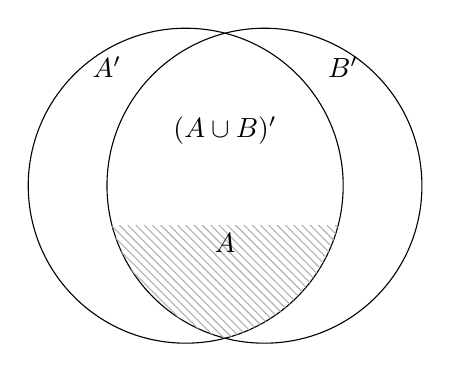
\begin{tikzpicture}[scale=1]
      % Draw the circles
      \draw (0,0) circle (2cm) node at (-1,1.5) {$A'$};
      \draw (1,0) circle (2cm) node at (2,1.5) {$B'$};

      % Shade the bottom portion of the intersection
      \begin{scope}
        \clip (0,0) circle (2cm);
        \clip (1,0) circle (2cm);
        \fill[pattern=north west lines, pattern color=gray!60, opacity=1] (-1,-2) rectangle (2,-0.5);
      \end{scope}

      % Add label for the shaded area
      \node at (0.5,-0.725) {$\minO{A}$};

      % Add label in the intersection
      \node at (0.5,0.7) {$(A \cup B)'$};
    \end{tikzpicture}
  \end{center}
\end{proof}

% \begin{proof} We will show $\minO{A} \subseteq \minO{(A\cup B)}$ and $\minO{A} \supseteq \minO{(A\cup B)}$

%   $\minO{A} \subseteq \minO{(A\cup B)}$:

%   Let $g \in \minO{A}$
%   \begin{enumerate}
%     \item $\minO{A} \subseteq A'$ \hfill  (Definition of minimisation)
%     \item $\minO{A} \subseteq B'$ \hfill (Given $A \twiddle B$)
%     \item $\minO{A} \subseteq (A \cup B)'$ \hfill (1,2, Lemma 3.3)
%           % \item $B \subseteq g'$ \hfill (4, Given $g \in \minO{A}$)
%     \item $\nexists h \in A'$ such that $ h < g$ \hfill (Definition of $\minO{A}$)
%           % \item $\nexists h \in G$ such that $h < g$ and $A \subseteq h'$ \hfill (5,6, By construction of $\minO{A}$)
%           % \item $\forall a \in \minO{(A \cup B)}, a \in A'$ \hfill(Definition of $\minO{(A\cup B)}$)
%     \item $\minO{(A\cup B)} \subseteq (A \cup B)' \subseteq A'$ \hfill (See)
%     \item $\nexists a \in \minO{(A \cup B)}$ with $a < g$ \hfill (4,5)
%     \item $g \in (A \cup B)'$ \hfill (Given: $g\in \minO{A}$, 3)
%           % \item $\minO{(A \cup B)} \subseteq (A \cup B)'$ \hfill (Definition of minimisation)
%     \item $g \in \minO{(A \cup B)}$ \hfill (6,7, Definition of $\minO{(A \cup B)}$)
%     \item $g$ is an arbitray element in $\minO{A}$, so $\minO{A} \subseteq \minO{(A \cup B)}$
%   \end{enumerate}

%   $\minO{A} \supseteq \minO{(A\cup B)}:$

%   Let $g \in \minO{(A \cup B)}$
%   \begin{enumerate}
%     \item $\minO{A} \subseteq B'$ \hfill (Given $A\twiddle B$)
%     \item $\minO{A} \subseteq A'$ \hfill (Definition of minimisation)
%     \item $\minO{A} \subseteq (A\cup B)'$ \hfill (1,2, Lemma 3.3)
%     \item $\nexists h \in (A \cup B)'$ such that $h < g$ \hfill (Definition of $\minO{(A \cup B)}$)
%     \item $\nexists a \in \minO{A}$ such that $a < g$ \hfill (3,4)
%   \end{enumerate}

% \end{proof}

\begin{equation}
  \frac{A \twiddle B, A \twiddle C}{(A \cup B) \twiddle C} \qquad \textbf{(Cautious Monotonicity)}
\end{equation}

\begin{proof}
  Let $A, B, C \subseteq M$.
  \begin{enumerate}
    \item $\minO{A} \subseteq A'$ \hfill (Definition of minimisation operator)
    \item $\minO{A} \subseteq B'$ \hfill (Given: $A \twiddle B$)
    \item $\minO{A} \subseteq C'$ \hfill (Given: $A \twiddle C$)
    \item $\minO{A} \subseteq (A \cup B)' $ \hfill (1,2, Lemma 3.3)
    \item $\minO{A} \subseteq (A \cup C)' $ \hfill (1,3, Lemma 3.3)
    \item $\minO{A} = \minO{(A\cup B)}$ \hfill (4, Lemma 3.5)
    \item $\minO{A} = \minO{(A \cup C)}$ \hfill (5, Lemma 3.5)
    \item $\minO{(A\cup C)} \subseteq (A \cup C)'$ \hfill (Definition of minimisation)
    \item $\minO{(A\cup B)} \subseteq (A\cup C)'$ \hfill (6,7,8)
    \item $(A\cup B) \twiddle C$ \hfill (9 is definition of this implication)
  \end{enumerate}
\end{proof}

\begin{remark}
  Cautious monotonicity stipulates that when given new information, if that information could have been inferred before, then it should not be inconsistent with earlier inferences. Monotonicity requires that any new knowledge not invalidate existing knowledge; CM weakens this requirement to be that only pieces of knowledge inferred from the same existing knowledge should not invalidate one another.
\end{remark}

\begin{equation}
  \frac{A \twiddle B, A \ntwiddle \neg C}{A \cup C \twiddle B} \qquad \textbf{(Rational Monotonicity)}
\end{equation}

\clearpage
\section{Minimal Concepts}
\subsection{Using the minimisation operator to define minimal concepts}
In the standard case, a concept of some formal context $\mathbb{K}$ is a pair $(A,B)$ where $A' = B$ and $A = B'$ where $A\subseteq G$ and $B\subseteq M$. We can also see that for some $B \subseteq M$, $(B', B'')$ is a formal concept.

Using the minimisation operator, we introduce a \textit{minimal formal concept} $(A,B)$ with $A = \minO{B}$ and $A' = B$. That is, a minimal formal concept $(A,B)$ is a formal concept where the set of minimal objects which have $B$ in their intent are precisely $A$, and the intersection of object intents of all objects in $A$ is precisely the set $B$.

\subsection{Ordering on minimal concepts}

If $(A_1, B_1)$ and $(A_2, B_2)$ are concepts of a formal context, $(A_1,B_1)$ is a subconcept $(\leq)$ of $(A_2, B_2)$ provided that $A_1 \subseteq A_2$ (equivalently, $B_1 \supseteq B_2)$.

\section{Questions}
\subsection{Is every material implication a defeasible implication?}
If we have a defeasible formal context $\K = (G,M,I,<)$ where $A,B\subseteq M$ and $A\rightarrow B$ is a valid implication over $M$, does $A \twiddle B$ hold in $\K$?

\bibliographystyle{IEEEtran}
\bibliography{references}  % the name of your .bib file
\end{document}
